%!TEX TS-program = xelatex
%!TEX encoding = UTF-8 Unicode

\documentclass[12pt]{extarticle}
% extarticle is like article but can handle 8pt, 9pt, 10pt, 11pt, 12pt, 14pt, 17pt, and 20pt text

\def \ititle {Origins of Mind}
 
\def \isubtitle {Lecture 02}
 
\def \iauthor {Stephen A. Butterfill}
\def \iemail{s.butterfill@warwick.ac.uk}
\date{}

%for strikethrough
\usepackage[normalem]{ulem}

\input{$HOME/Documents/submissions/preamble_steve_handout}

%\bibpunct{}{}{,}{s}{}{,}  %use superscript TICS style bib
%remove hanging indent for TICS style bib
%TODO doesnt work
\setlength{\bibhang}{0em}
%\setlength{\bibsep}{0.5em}


%itemize bullet should be dash
\renewcommand{\labelitemi}{$-$}

\begin{document}

\begin{multicols}{3}

\setlength\footnotesep{1em}


\bibliographystyle{newapa} %apalike

%\maketitle
%\tableofcontents




%--------------- 
%--- start paste
\def \ititle {Origins of Mind}
 
\def \isubtitle {Lecture 03}
 
 
 
\
 
 
 
\begin{center}
 
{\Large
 
\textbf{\ititle}: \isubtitle
 
}
 
 
 
\iemail %
 
\end{center}
 
 
 
\section{Perception of Causation}
 
‘There are some cases … in which a causal impression arises, clear, genuine, and unmistakable, and the idea of cause can be derived from it by simple abstraction in just the same way as the idea of shape or movement can be derived from the perception of shape or movement’
\citep[p.\ 270--1]{Michotte:1946nz}
 
Infants at around six months of age seem also to distinguish launching from other sequences, much as adults do \citep{Leslie:1987nr}.
 
‘when there is a launching event beneath the overlap (or underlap event) timed such that the launch occurs at the point of maximum overlap, observers inaccurately report that the overlap is incomplete, suggesting that they see an illusory crescent.’
\citep[p.\ 461]{Scholl:2004dx}
 
Why does the illusory causal crescent appear? Scholl and Nakayama suggest a
 
‘a simple categorical explanation for the Causal Crescents illusion: the visual system, when led by other means to perceive an event as a causal collision, effectively ‘refuses’ to see the two objects as fully overlapped, because of an internalized constraint to the effect that such a spatial arrangement is not physically possible. As a result, a thin crescent of one object remains uncovered by the other one-as would in fact be the case in a straight-on billiard-ball collision where the motion occurs at an angle close to the line of sight.’
\citep[p.\ 466]{Scholl:2004dx}
 
‘just as the visual system works to recover the physical structure of the world by inferring properties such as 3-D shape, so too does it work to recover the causal … structure of the world by inferring properties such as causality’
\citep[p.\ 299]{Scholl:2000eq}
 
 
 
\section{Object Indexes and Causal Interactions}
 
The \emph{object-specific preview effect}: ‘observers can identify target letters that matched the preview letter from the same object faster than they can identify target letters that matched the preview letter from the other object.’
\citep[p.\ 2]{Krushke:1996ge}
 
 
 
\section{Object Indexes and the Principles of Object Perception}
 
The principles of object perception
are not items of knowledge
instead
they characterise the operation of
object-indexes (aka FINSTs, mid-level object files)
\citep{Leslie:1998zk,Scholl:1999mi,Carey:2001ue}.
 
 
 
\section{Perceptual Expectations}
 
\begin{center}
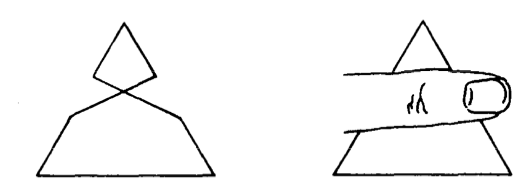
\includegraphics[scale=0.3]{img/kellman_1983_fig2.neg.png}
\end{center} 
\emph{source}: Michotte et al (1964) via Kellman and Spelke (1983, figure 2) 
%--- end paste
%--------------- 
 
\footnotesize 
\bibliography{$HOME/endnote/phd_biblio}

\end{multicols}

\end{document}